\textbf{Цель работы:} исследование кривых намагничивания ферромагнетиков с помощью баллистического гальванометра.

\textbf{В работе используются:} генератор токов намагничивания (ГТН), тороид, соленоид, баллистический гальванометр с осветителем и шкалой, мультиметр-амперметр, лабораторный автотрансформатор (ЛАТР), разделительный трансформатор, ключи, переключатели.
                    
\section{Теоретическое введение}
	
Ферромагнетики -- вещества, которые при определенной температуре обладают самопроизвольной намагниченностью $\boldsymbol{M}$ в отсутствие внешнего магнитного поля. В ферромагнетиках образуются отдельные намагниченные области – домены (от $10^{-2}$ до $10^{-6}$ см$^3$), магнитные моменты в которых ориентируются параллельно.

Зависимость вектора магнитной индукции $\boldsymbol{B}$ ферромагнетика от вектора напряжённости магнитного поля $\boldsymbol{H}$ нелинейна. В системе СИ эта связь имеет вид
\begin{equation} 
    \label{eq:BM}
    \boldsymbol{B} = \mu_0(\boldsymbol{H} + \boldsymbol{M})
\end{equation}

При этом намагниченность зависит не только от состояния вещества, а также от его предудущих состояний, то есть зависимость $\boldsymbol{B}(\boldsymbol{H})$ не является функцией состояния. График этой зависимости изображён на рис. 1.

\begin{figure}[h!]
    \center{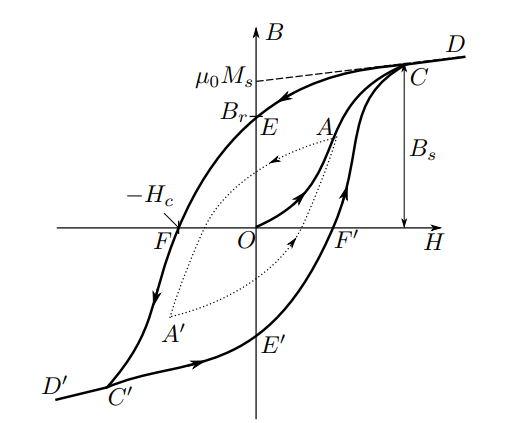
\includegraphics[width = 9 cm]{images/1.png}}
    \caption{Петля гистерезиса ферромагнетика}
    \label{ris:hysteresis}
\end{figure}

Измерить эту зависимость можно следующим способом: На тороидальный сердечник (рис. 2), изготовленный из исследуемого образца, равномерно намотана намагничивающая обмотка с числом витков $N$, а поверх неё — измерительная обмотка с числом витков $N'$. При скачкообразном изменении тока в намагничивающей обмотке в измерительной
обмотке возникает ЭДС индукции. Ток, вызванный этой ЭДС, регистрируется гальванометром $\text{Г}$, работающим в баллистическом (импульсном) режиме: его отклонение пропорционально полному заряду $\Delta q$, протекшему через него.

\begin{figure}[h!]
    \centering
    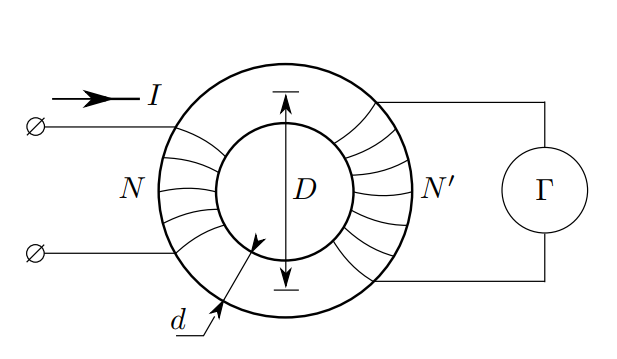
\includegraphics[width = 7 cm]{images/2.png}
    \caption{Схема для измерения индукционного тока}
    \label{ris:ust1}
\end{figure}

Напряжённость поля $H$ в сердечнике пропорциональна току $I$ в первичной (намагничивающей) обмотке, а изменение магнитной индукции $\Delta B$ — заряду $\Delta q$, протекшему через вторичную (измерительную) обмотку. Таким образом, измеряя токи $\Delta I$ и суммируя отклонения $\Delta q$ гальванометра $\text{Г}$, можно получить зависимость $B(H)$ для материала сердечника.

Напряжённость магнитного поля в тороиде равна 

\begin{equation}
    \label{eq:H}
    H = \frac{N}{\pi D} I
\end{equation}

Гальванометр измеряет протёкший чеерез него заряд баллистическим методом, то есть

\begin{equation}
    \Delta x = \frac{\Delta q}{b}
\end{equation}

Учитывая, что заряд возникает из-за тока электромагнитной индукции, получим

\begin{equation}
    \Delta x = \frac{S_t N'}{b R_t} \Delta B 
\end{equation}

Здесь $R_t$ -- полное сопротивление измерительной цепи тороида, $S_{t}$ -- площадь поперечного сечения тороида.

Баллистическую постоянную $b$ можно определить с помощью следующей схемы (рис. 3): вместо тороида возьмём соленоид, и, всользовавшись той же формулой, получим

\begin{equation}
    \Delta x = \frac{S_c N_c'}{bR_c} \Delta B_c = \frac{\mu_0 S_c N_c' N_c}{b R_c l_c} \Delta I_c
\end{equation}

\begin{figure}[h]
    \centering
    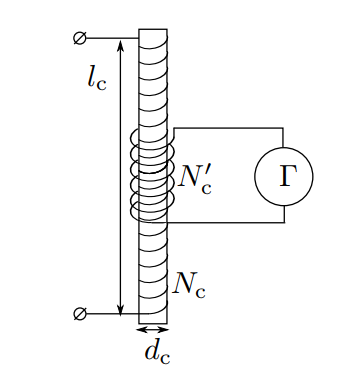
\includegraphics[width = 6 cm]{images/3.png}
    \caption{Схема для калибровки
    гальванометра}
    \label{kalibr}
\end{figure}

Таким образом, можно исключить калибровочную постоянную $b$, учитывая, что в исследуемой схеме будет подобраны сопротивления схем с тороидом и соленоидом были равны.

\begin{equation}
    \label{eq:B}
    \Delta B = \mu_0 \left(\frac{d_c}{d_t}\right)^2 \frac{N_{c}'}{N'} \frac{N_{c}}{l_c} \Delta I_c \frac{\Delta x}{\Delta x_c}
\end{equation}

Схема для исследования петли гистерезиса представлена на рис. 4.

\begin{figure}[h]
    \centering
    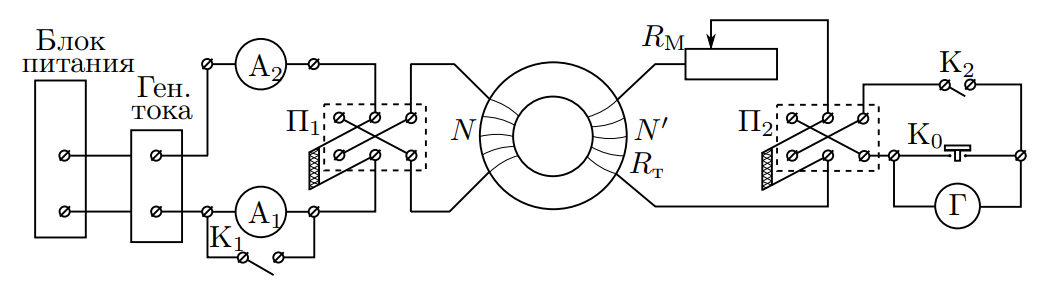
\includegraphics[width = 13 cm]{images/4.png}
    \caption{Схема установки для исследования петли гистерезиса}
    \label{}
\end{figure}

Здесь $R_m$ -- сопротивление нагрузки для контроля амплитуды отклонения луча (работа гальванометра реализована через лампу, чтобы можно было исследовать отклонение луча, зависящего от пройденного заряда).

Для калибровочной постоянной нужно собрать такую же схему, где вместо тороида следует поместить соленоид.


\section{Ход работы}

Для начала соберём нужны данные для дальнейшего исследования. $N_t = 1750$, $N' = 300$, $R_0 = 5,6$ Ом (сопротивление гальванометра).

Собрав схему и настроив гальванометр, обойдём всю кривую гистерезиса, исследуя, какое значение сопротивления $R_m$ нужно подобрать, чтобы отклонение луча не заходило за пределы измерительной шкалы. Получим $R_m = 220$ Ом.

\subsection{Предельная петля гистерезиса}

Начнём измерять предельную петлю гистерезиса с максимального тока (тока насыщения), равного $I_0 = 1,7 \pm 0,02$ А. 

Результаты измерений зависимости $\Delta B(I)$ находятся в приложении к отчёту лабораторной работы.

\subsection{Калибровка гальванометра}  

Подсоединив соленоид вместо тороида найдём значения $\Delta I_c = 1,71 \pm 0,02$ А и $x_c = 13,5 \pm 0,2$ см. Здесь учтена погрешность измерения отклонения луча, в которую входит погрешность определения нулевой точки луча и точки измерения.

Характеристика соленоида: $N_c' = 500$, $N_c = 940$, $R_c = 46$ Ом, $l_c = 0,8$ м, $d_c= 0,07$ м.

\subsection{Начальная кривая намагничивания} 

Теперь с помощью генератора переменного тока, уменьшая амплитуду тока но нуля, вернём тороид в начальное состояние $(0,0)$ в зависимости $H(B)$, иначе говоря, размагнитим.

Теперь проведём такие же измерения, как и для предельной петли, дойдя до тока насыщения. 

\subsection{Обработка данных}  

Для начала, учитывая зависимость напряжённости магнитного поля и силы тока намагничивающей обмотки, переведём все значени сил тока в напряжённость (с учётом знаков напряжённости):

\begin{equation}
    H = \frac{N_t}{\pi D} I
\end{equation}

Средний диаметр тороида равен $D = 0,1$ м, откуда находим $H$.

Теперь, используя формулу ниже, переведём значения $\Delta x$ в значения $\Delta B$ как для предельной петли, так и для начальной кривой.

\begin{equation}
    \label{eq:B2}
    \Delta B = \mu_0 \left(\frac{d_c}{d_t}\right)^2 \frac{N_{c}'}{N'} \frac{N_{c}}{l_c} \Delta I_c \frac{\Delta x}{\Delta x_c}
\end{equation}

Здесь $d_t = 0,01$ м, остальные значения уже известны.

Просуммировав изменения индукции для начальной кривой на каждом шаге, получим максимальное значение индукции $B_{max} = 1,35 \pm 0,04$, через которое с помощью значений $\Delta B$ можно найти все остальные значения индукции.

Построим по всем точкам петлю гистерезиса (см рис. 5).

\begin{figure}[h!]
    \centering
    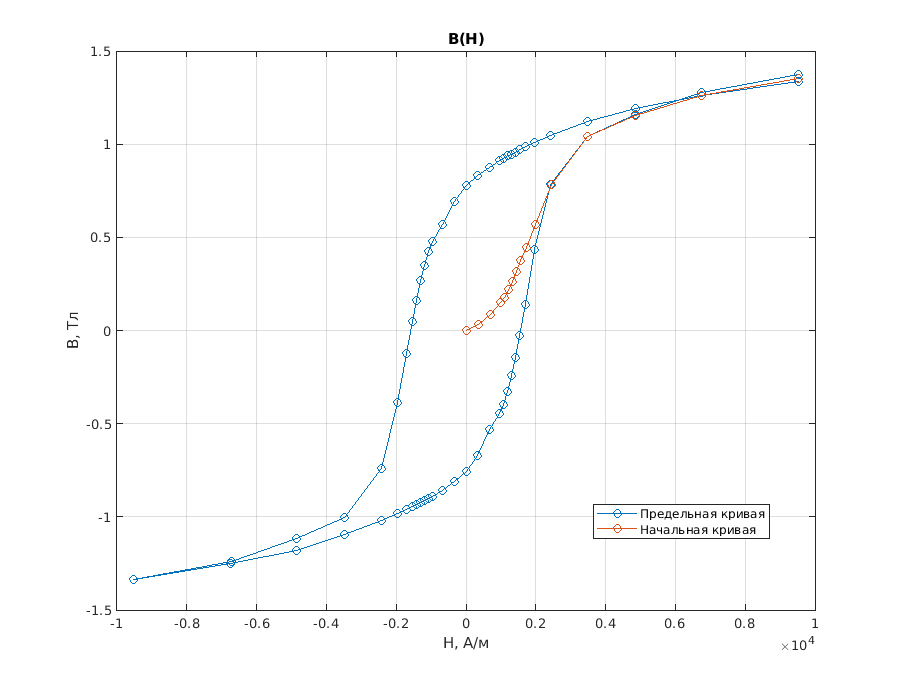
\includegraphics[width = 14 cm]{images/gist.png}
    \caption{График петли гистерезиса}
    \label{gist}
\end{figure}

Найдём из графика оценку коэрцитивной силы стали (исследуемого материала) $H_c = 1540 \pm 20 \; A/\text{м}$ (точность высока, т.к. высока точность измерений сил тока). 

Также найдём индукцию насыщения $B_s = 1,37 \pm 0,05$ Тл.

По наклону графика определим значение максимальной дифференциальной магнитной проницаемости $\mu = \frac{1}{\mu_0} \frac{dB}{dH} = 533 \pm 21$. 

Заметим, что значения по порядку сходятся со справочными $\mu = 1100$ (если материал -- чистая мягкая сталь) и $H_c = 1540 \pm 20 \; A/\text{м}$ (если сталь углеродистая).

\section{Заключение}

Для стали действительно справедлива ферромагнитная теория, так как зависимость $B(H)$ имеет вид петли гистерезиса. Значения коэрцитивной силы, индукции насыщения и дифференциальной магнитной проницаемости зависят полностью от сплава стали, которай является исследуемым в этом эксперименте материалом. Для полученных значений определить сплав стали не удалось из-за расхождений в одном из показателей, но по порядку величин значения сходятся.




























